\section*{Условие задания}

Согласно порядковому номеру в списке 13 принимаем схему I и номер варианта 7.

\begin{figure}[H]
    \begin{center}
        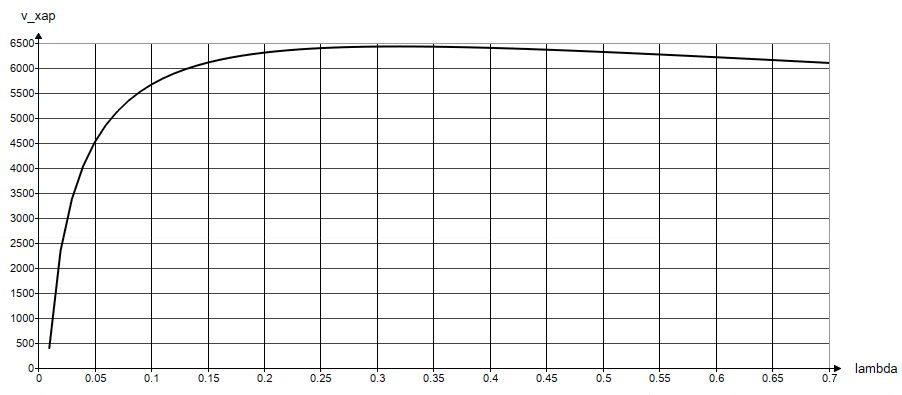
\includegraphics[width = 0.9\linewidth]{pic1.PNG}
        \caption*{Рисунок 1 --- Схема ракеты}
        \label{pic1}
    \end{center}
\end{figure}

Исходные данные:
\begin{itemize}
    \item Координаты сечения 
        \begin{itemize}
        \item $x_1 = 1.7$ м
        \item $x_2 = 3.5$ м
        \item $x_3 = 4.0$ м
        \item $x_4 = 7.0$ м
        \item $x_5 = 10.0$ м
        \item $x_6 = 11.0$ м
        \item $x_7 = 15.0$ м
        \item $x_8 = 19.0$ м
        \item $x_9 = 21.0$ м
    \end{itemize}
    \item Параметры АС
        \begin{itemize}
            \item $w_0 = 25$
            \item $w_\t{р} = 70$
            \item $W_{2\t{р}} = 110$
            \item $k_\t{р} = 0.6$
        \end{itemize}
    \item $M_1 = 2.0$ т
    \item $M_2 = 2.0$ т
    \item $J_0 = 3.0 \; \t{т} \cdot \t{м}^2$
    \item $x_\t{ГП} = 19.5$ м
\end{itemize}

Требуется:
\begin{enumerate}
    \item Для заданного варианта определить две первых собственные частоты упругих поперечных колебаний корпуса ракеты.
    \item Построить эпюры формы упругой линии и угла поворота сечений для каждого тона колебаний сечения.
    \item Построить эпюры изгибающих моментов и поперечных сил.
    \item Выполнить пункты №1 и №2 для полностью заправленной ракеты (момент старта) и <<сухой>> ракеты (момент выключения ДУ при стрельбе на максимальную дальность).
    \item Вычислить значения приведенных масс для расчетных случаев.
\end{enumerate}

\section{Решение}

Решать задачу будем с помощью метода начальных параметров. Для этого распределим сосредоточенную массу в окрестности точки, в которой она расположена на расстоянии $0.1 \; \t{м}$ в обе стороны. Дифференциальное уравнение поперечных колебаний для i-го участка имеет вид
\begin{equation}
    \label{eq1}
    EJ_i \cdot f_i^{IV} (x) - \omega^2 m_i f_i(x) = 0
\end{equation}

Введем коэффициент колебаний $b_i$:
\begin{equation}
    \label{eq2}
    b_i^4 = \frac{\omega^2 m_i}{EJ_i}
\end{equation}

Тогда уравнение колебаний (\ref{eq1}) примет вид:
\begin{equation}
    \label{eq3}
    f_i^{IV}(x) - b_i^4 f_i(x) = 0
\end{equation}

Решение системы уравнений (\ref{eq3}) должно удовлетворять граничным условиям и условиям сопряжения участков стержня. Данная задача разрешима только для тех значений $\omega$, которые являются частотами свободных колебаний неоднородного стержня. Решение уравнений (\ref{eq3}) представим в виде линейной комбинации балочных функций Крылова:
\begin{equation}
    \label{eq4}
    f_i(x) = C_{1i} S(b_ix) + C_{2i} T(b_ix) + C_{3i} U(b_ix) + C_{4i} V(b_ix)
\end{equation}
где балочные функции Крылова имеют вид
\begin{equation}
    \label{eq5}
    \begin{split}
        S(b_ix) = \frac{1}{2}(ch(b_ix) + \cos(b_ix))
        \\
        T(b_ix) = \frac{1}{2}(sh(b_ix) + \sin(b_ix))
        \\
        U(b_ix) = \frac{1}{2}(ch(b_ix) - \cos(b_ix))
        \\
        V(b_ix) = \frac{1}{2}(sh(b_ix) - \sin(b_ix))
    \end{split}
\end{equation}

Функции Крылова обладают свойствами, делающими их удобными для решения задач поперечных колебаний стержня:
\begin{enumerate}
    \item $S(0) = 1; \; T(0) = U(0) = V(0) = 0$
    \item $S'(b_ix) = b_iV(b_ix); \; V'(b_ix) = b_iU(b_ix); \; U'(b_ix) = b_iT(b_ix); \; T'(b_ix) = b_iS(b_ix)$
\end{enumerate}

Введем вектор формы колебаний:
\begin{equation}
    \label{eq6}
    \overline{u}_i(x) = 
    \begin{bmatrix}
        u_{1i}(x)
        \\
        u_{2i}(x)
        \\
        u_{3i}(x)
        \\
        u_{4i}(x)
    \end{bmatrix}
\end{equation}
где:
\begin{itemize}
    \item $u_{1i}(x) = f_i(x)$ --- форма перемещений
    \item $u_{2i}(x) = f'_i(x)$ --- форма угла поворота
    \item $u_{3i}(x) = EJ_i \cdot f''_i(x)$ --- форма изгибающего момента
    \item $u_{4i}(x) = EJ_i \cdot f'''_i(x)$ --- форма поперечного момента
\end{itemize}

Так как на стыках меняется только значения погонных масс и жесткостей, то условие стыка примет вид
\begin{equation}
    \label{eq7}
    \overline{u}_i(l_i) = \overline{u}_{i+1}(0)
\end{equation}

Исходя из свойств функций Крылова, можно связать между собой вектор формы в любой точке участка с вектором формы в его начале. Это условие связи имеет вид
\begin{equation}
    \label{eq8}
    \overline{u}_i(x) = A_i(x) \cdot \overline{u}_i(0)
\end{equation}
где матрица $A$ имеет вид
\begin{equation}
    \label{eq9}
    A_i(x) = 
    \begin{bmatrix}
        S(b_ix) & \displaystyle \frac{T(b_ix)}{b_i} & \displaystyle \frac{U(b_ix)}{EJ_i \cdot b_i^2} & \displaystyle \frac{V(b_ix)}{EJ_i \cdot b_i^3}
        \\[10pt]
        V(b_ix) \cdot b_i & S(b_ix) & \displaystyle \frac{T(b_ix)}{EJ_i \cdot b_i} & \displaystyle \frac{U(b_ix)}{EJ_i \cdot b_i^2}
        \\[10pt]
        EJ_i \cdot b_i^2 \cdot U(b_ix) & V(b_ix) \cdot EJ_i \cdot b_i & S(b_ix) & \displaystyle \frac{T(b_ix)}{b_i}
        \\[10pt]
        EJ_i \cdot b_i^3 \cdot V(b_ix) & EJ_i \cdot b_i^2 \cdot U(b_ix) & V(b_ix) \cdot b_i & S(b_ix)
    \end{bmatrix}
\end{equation}

Из условия (\ref{eq7}) следует
\begin{equation}
    \label{eq10}
    \overline{u}_{i+1}(x) = A_{i+1}(x) \cdot A_i(l_i) \cdot\overline{u}_i(0)
\end{equation}

Поэтому решение для произвольного участка можно выразить через вектор формы в начале первого участка:
\begin{equation}
    \label{eq11}
    \overline{u}_i(x) = A_i(x) \cdot \left( \prod_{j=1}^{i-1} A_j(l_j) \right) \cdot \overline{u}_1(0)
\end{equation}

Введем матрицу $P$:
\begin{equation}
    \label{eq12}
    P = \prod_{j=1}^{k} A_j(l_j)
\end{equation}

Тогда выражение (\ref{eq11}) примет вид
\begin{equation}
    \label{eq13}
    \overline{u}_i(L) = P \cdot \overline{u}_i(0)
\end{equation}
или в скалярной форме:
\begin{equation}
    \label{eq14}
    u_r(l) = \sum_{s=1}^{4} p_{rs} u_s(0)
\end{equation}
где $p_{rs}$ --- коэффициенты матрицы $P$, зависящие от частоты свободных колебаний $\omega$.

Граничные условия на концах ракеты (свободные концы) будут иметь вид
\begin{equation}
    \label{eq15}
    \begin{cases}
        u_3(0) = 0
        \\
        u_4(0) = 0
        \\
        u_3(L) = 0
        \\
        u_4(L) = 0
    \end{cases}
\end{equation}

С учетом граничных условий (\ref{eq15}) выражение (\ref{eq14}) примет вид
\begin{equation}
    \label{eq16}
    \begin{cases}
        u_1(L) = p_{11} u_1(0) + p_{12} u_2(0)
        \\
        u_2(L) = p_{21} u_1(0) + p_{22} u_2(0)
        \\
        0 = p_{31} u_1(0) + p_{42} u_2(0)
        \\
        0 = p_{41} u_1(0) + p_{42} u_2(0)
    \end{cases}
\end{equation}

Нетривиальным решением системы (\ref{eq16}) явлется выражение
\begin{equation}
    \label{eq17}
    p_{31} \cdot p_{42} - p_{32} \cdot p_{41} = 0
\end{equation}